\subsection{Source Code Repository}
The source code for this dissertation, including data preprocessing scripts, model training code, and results visualization
is available in a public GitHub repository at \url{https://github.com/codecZeus/xgb_on_cicids2017_in_nids}. This repository is intended to 
facilitate reproducibility and further research in the field of network intrusion detection.


\subsection*{XGBoost on CIC-IDS2017 in NIDS pipeline outputs}
\begin{figure}[H]
     \centering
     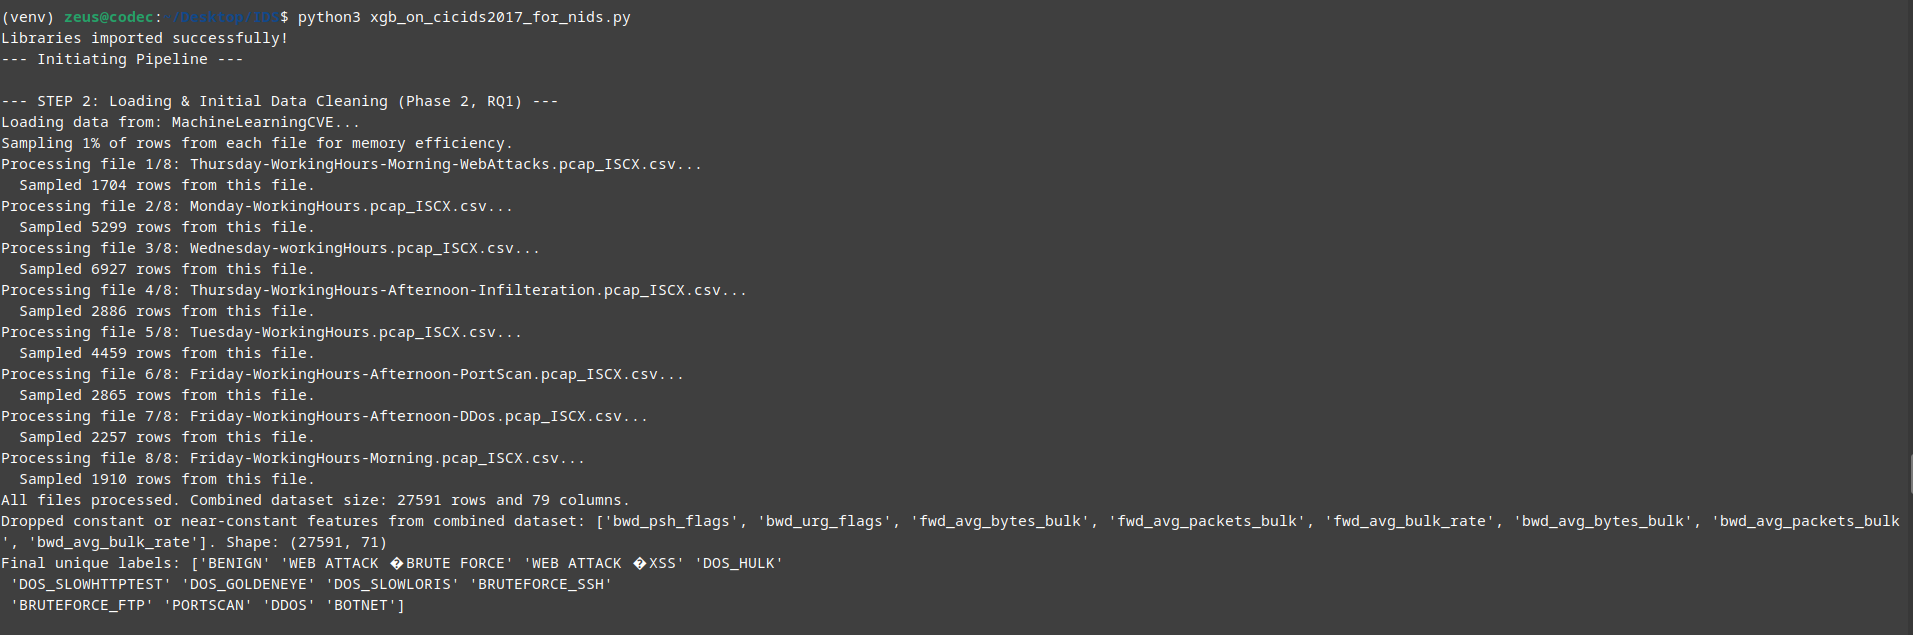
\includegraphics[width=0.75\textwidth]{assets/figures/outputs/1.png}
     \caption{Data loading and initial data cleaning phase}
     \label{fig:number_of_samples_per_category_initial_dataset} 
 \end{figure}

 \begin{figure}[H]
     \centering
     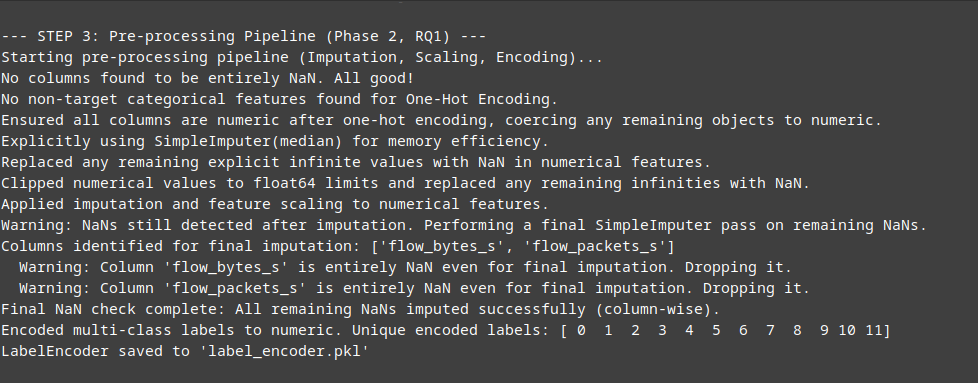
\includegraphics[width=0.75\textwidth]{assets/figures/outputs/2.png}
     \caption{Data pre-processing pipeline phase}
     %\label{fig:whatwebb} 
 \end{figure}
 
 \begin{figure}[H]
     \centering
     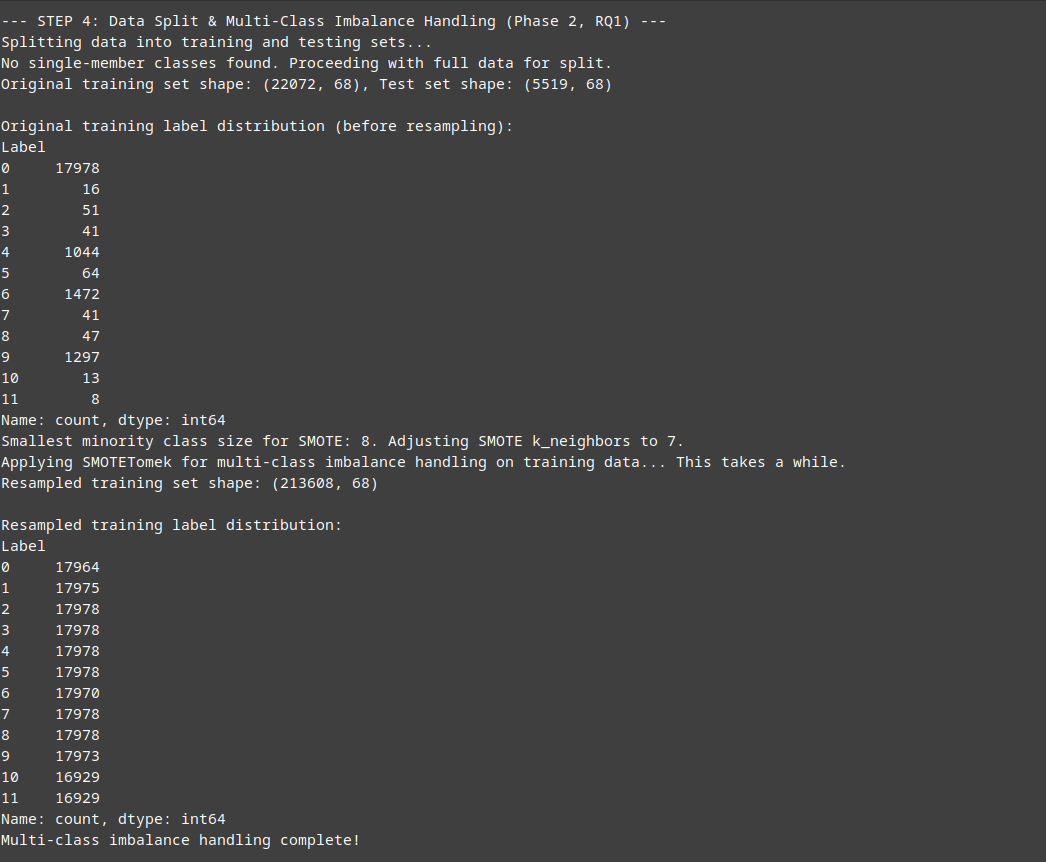
\includegraphics[width=0.75\textwidth]{assets/figures/outputs/3.png}
     \caption{Data split and multi class imbalance handling phase}
     %\label{fig:whatwebb} 
 \end{figure}
 
 \begin{figure}[H]
     \centering
     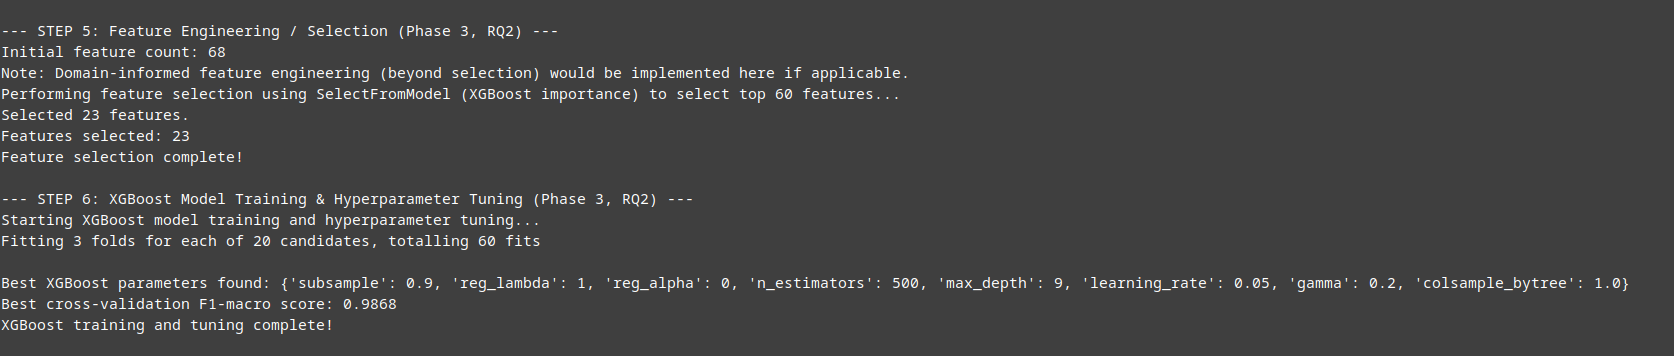
\includegraphics[width=0.75\textwidth]{assets/figures/outputs/4.png}
     \caption{Feature Engineering and XGBoost model training phase}
     \label{fig:xgboost_best_hp_search} 
 \end{figure}
 
 \begin{figure}[H]
     \centering
     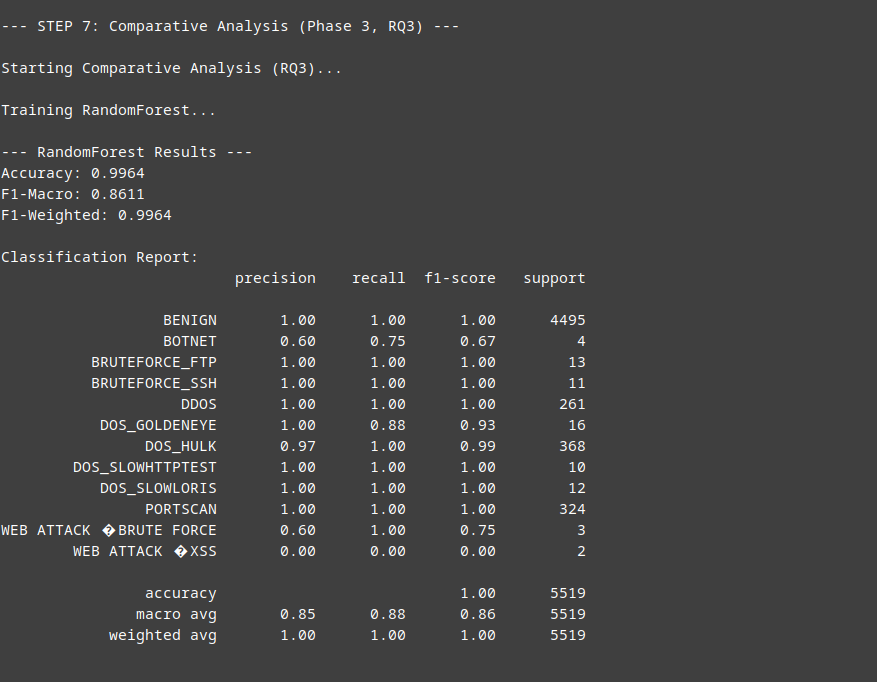
\includegraphics[width=0.75\textwidth]{assets/figures/outputs/5.png}
     \caption{Comparative analysis and F-1 score}
     \label{fig:f-1_score} 
 \end{figure}
 
 \begin{figure}[H]
     \centering
     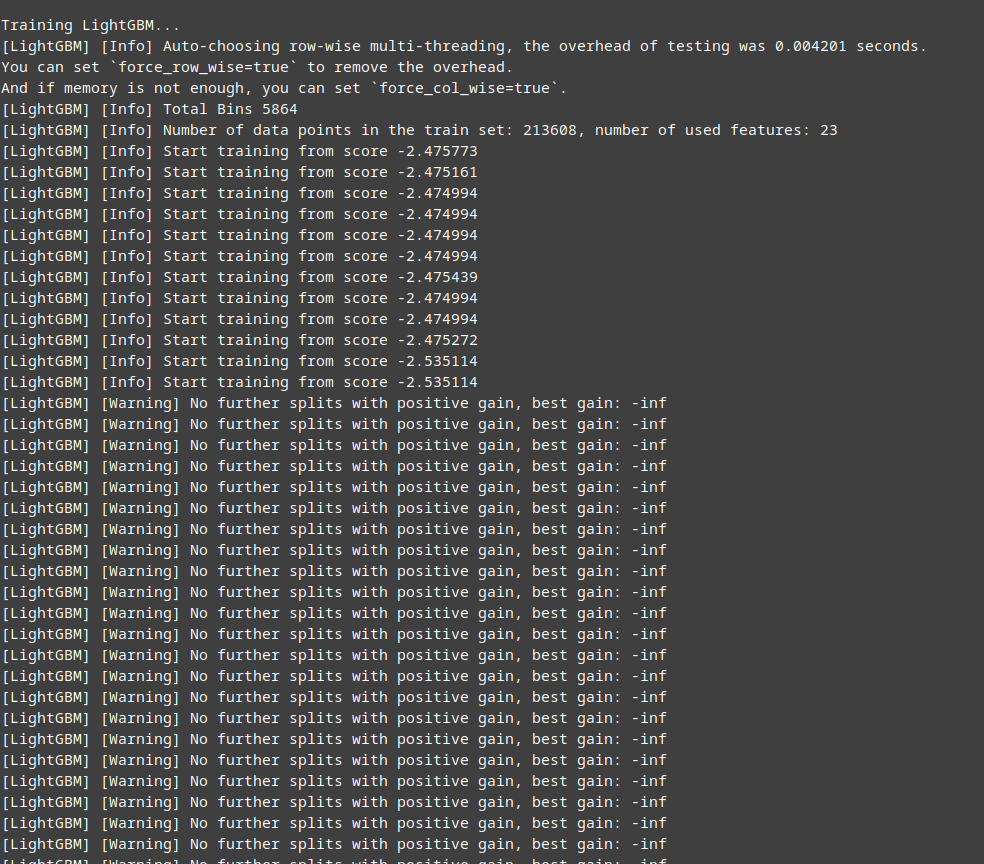
\includegraphics[width=0.75\textwidth]{assets/figures/outputs/6.png}
	\caption{Training LightGBM}
     %\label{fig:whatwebb} 
 \end{figure}
 
 \begin{figure}[H]
     \centering
     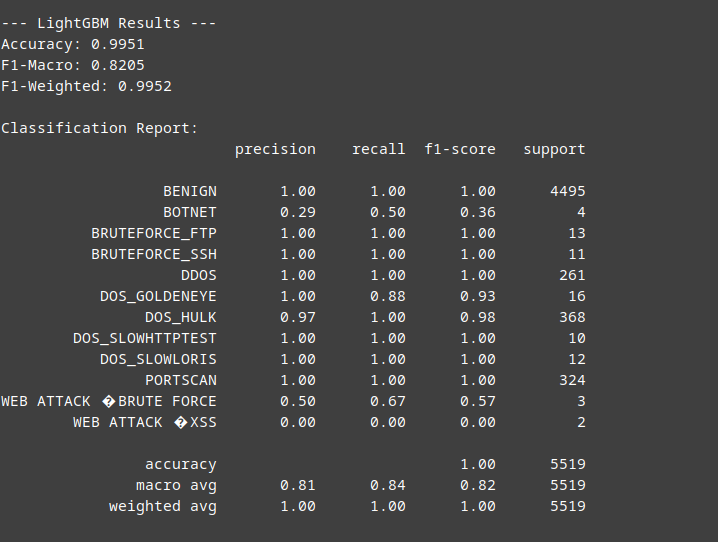
\includegraphics[width=0.75\textwidth]{assets/figures/outputs/7.png}
	\caption{LightGBM Results}
     %\label{fig:whatwebb} 
 \end{figure}
 
 \begin{figure}[H]
     \centering
     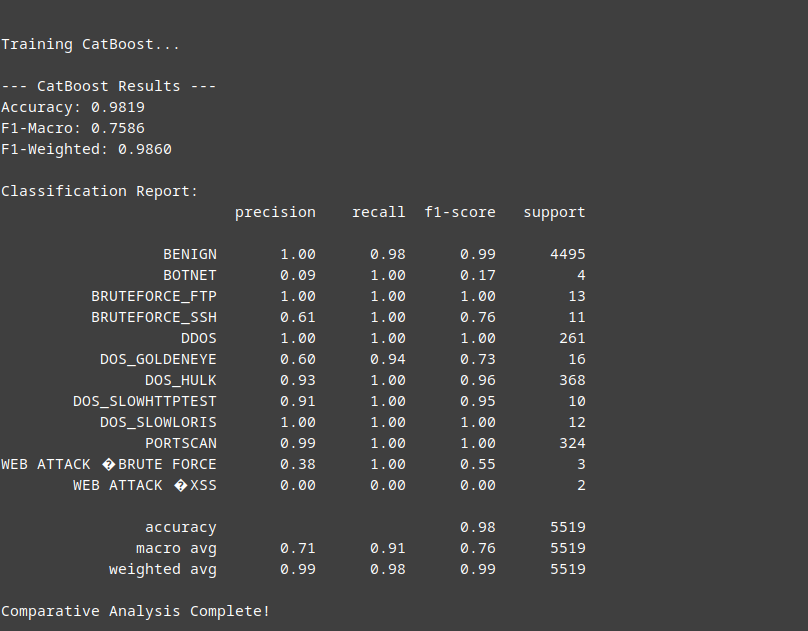
\includegraphics[width=0.75\textwidth]{assets/figures/outputs/8.png}
     \caption{Training CatBoost and its result}
     %\label{fig:whatwebb} 
 \end{figure}
 
 \begin{figure}[H]
     \centering
     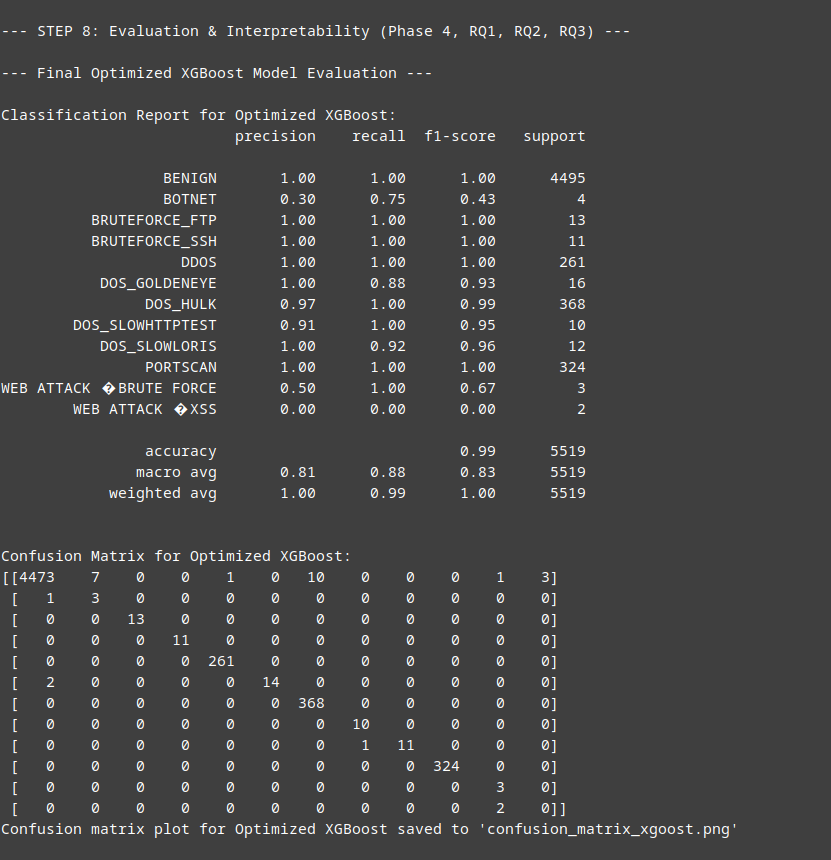
\includegraphics[width=0.75\textwidth]{assets/figures/outputs/9.png}
     \caption{Finial XGBoost Results}
     %\label{fig:whatwebb} 
 \end{figure}
 
 \begin{figure}[H]
     \centering
     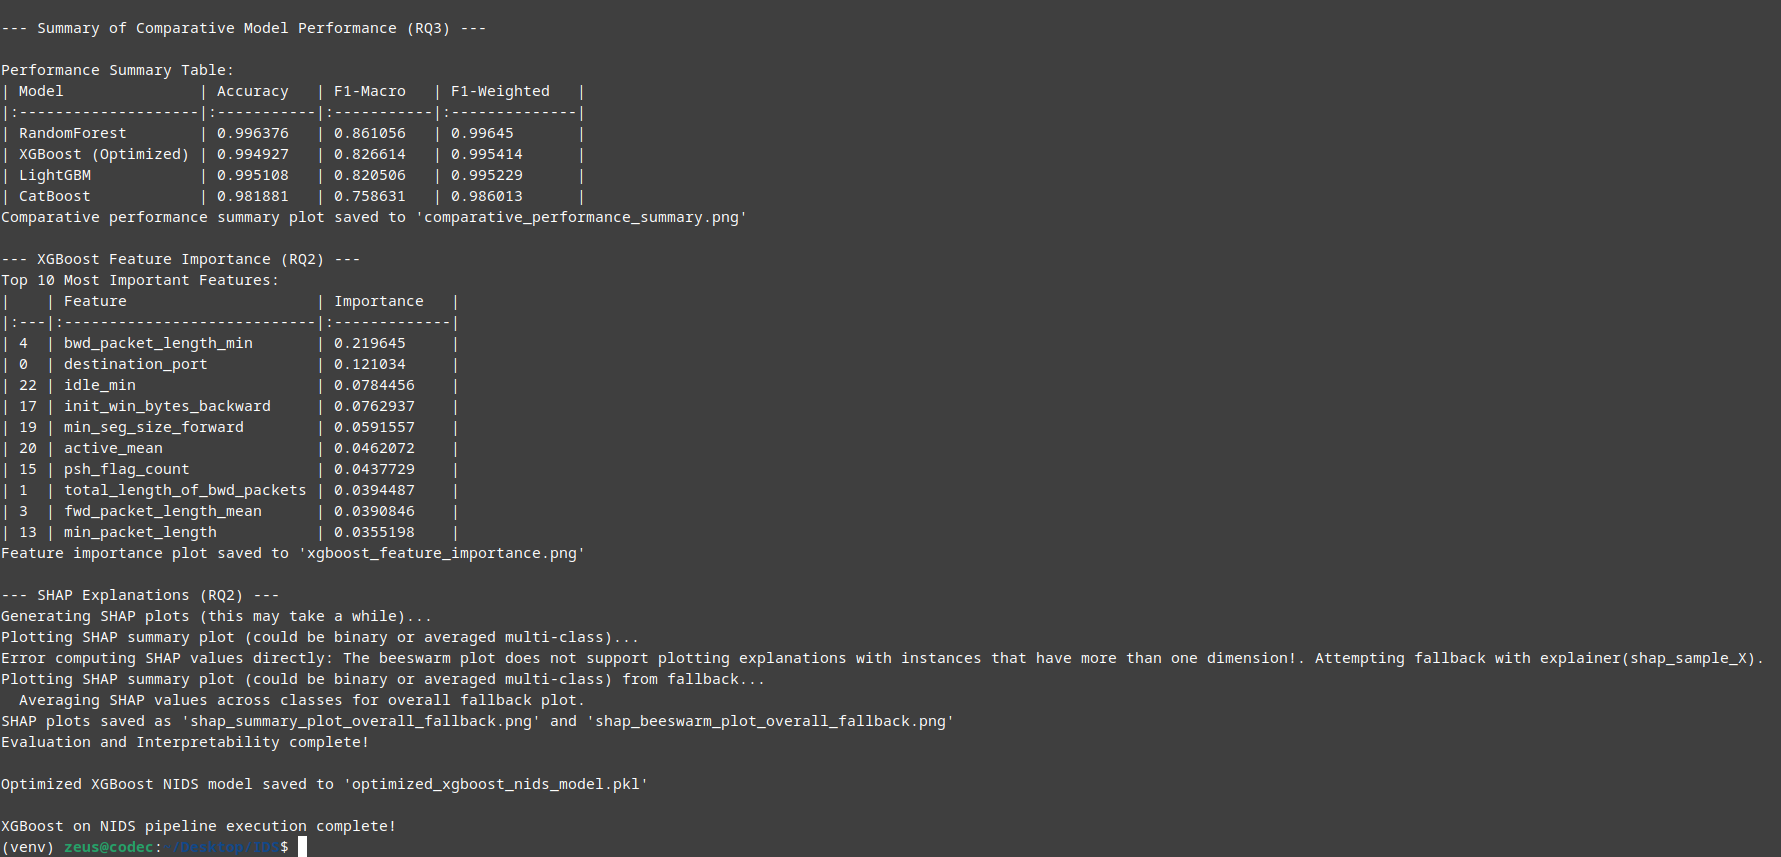
\includegraphics[width=0.75\textwidth]{assets/figures/outputs/10.png}
     \caption{Comparative analysis and evaluation graph generation phase}
     %\label{fig:whatwebb} 
 \end{figure}

% Define column types with wrapping
\newcolumntype{L}[1]{>{\raggedright\arraybackslash}p{#1}}
\newcolumntype{C}[1]{>{\centering\arraybackslash}p{#1}}
\newcolumntype{R}[1]{>{\raggedleft\arraybackslash}p{#1}}

\begin{longtable}{|L{6cm}|C{2cm}|C{2.5cm}|C{3cm}|C{2cm}|}
\caption{Dataset Features: Data Types, Null Values, Memory Usage, and Associated Commands}\label{tab:info} \\
\hline
\textbf{Feature} & \textbf{Data Type} & \textbf{Null Values} & \textbf{Memory Usage (RAM)} & \textbf{Command} \\
\hline
\endfirsthead

\hline
\textbf{Feature} & \textbf{Data Type} & \textbf{Null Values} & \textbf{Memory Usage (RAM)} & \textbf{Command} \\
\hline
\endhead

DestinationPort & int64 & 0 & 581MB & .info() \\ \hline 
Duration & float64 & 0 & 581MB & .info() \\ \hline 
Flow\textunderscore ID & int64 & 0 & 581MB & .info() \\ \hline 
Label & object & 2030 NaNs & 2.9MB & .info() \\ \hline 
Month & int64 & 0 & 581MB & .info() \\ \hline 
New\textunderscore Connections & int64 & 0 & 581MB & .info() \\ \hline 
Packet\textunderscore Direction & object & 0 & 581MB & .info() \\ \hline 
Packets\textunderscore In\textunderscore PerIOD & int64 & 0 & 581MB & .info() \\ \hline 
Packets\textunderscore Out\textunderscore PerIOD & int64 & 0 & 581MB & .info() \\ \hline 
Packet\textunderscore Size & int64 & 0 & 581MB & .info() \\ \hline 
Protocol & object & 0 & 581MB & .info() \\ \hline 
Source\textunderscore Flags & int64 & 0 & 581MB & .info() \\ \hline 
SourcePort & int64 & 0 & 581MB & .info() \\ \hline 
Total\textunderscore Flow\textunderscore Packet\textunderscore Count & int64 & 0 & 581MB & .info() \\ \hline 
Total\textunderscore Packet\textunderscore Length & float64 & 0 & 581MB & .info() \\ \hline 
Total\textunderscore FlowBytes\textunderscore Length & float64 & 0 & 581MB & .info() \\ \hline 
Year & int64 & 0 & 581MB & .info() \\ \hline 
FTP\textunderscore ORIGINALFERETSIZE & int64 & 0 & 581MB & .info() \\ \hline 
HTTPMethods & object & 0 & 581MB & .info() \\ \hline 
HTTPRequest\textunderscore Referer & object & 0 & 581MB & .info() \\ \hline 
HTTPRequest\textunderscore ResponseCode & object & 0 & 581MB & .info() \\ \hline 
HTTPRequest\textunderscore UserAgent & object & 0 & 581MB & .info() \\ \hline 
HTTPResponse\textunderscore Code & object & 0 & 581MB & .info() \\ \hline 
JSON\textunderscore JSON & object & 0 & 581MB & .info() \\ \hline 
Packet\textunderscore Sequence\textunderscore Number& int64 & 0 & 581MB & .info() \\ \hline 
SFTP\textunderscore OriginalFERETSIZE & int64 & 0 & 581MB & .info() \\ \hline 
SSLVersion & object & 0 & 581MB & .info() \\ \hline 
SSHCommand\textunderscore ID & int64 & 0 & 581MB & .info() \\ \hline 
SSHVersion & object & 0 & 581MB & .info() \\ \hline 
TLSTicketLifetime & float64 & 0 & 581MB & .info() \\ \hline 
FTPDataTransferSize & int64 & 0 & 581MB & .info() \\ \hline 
FTPCommandID & int64 & 0 & 581MB & .info() \\ \hline 
DNSQryName & object & 0 & 581MB & .info() \\ \hline 
DNSRR & object & 0 & 581MB & .info() \\ \hline 
Dst\textunderscore Land & object & 0 & 581MB & .info() \\ \hline 
Dst\textunderscore Lon & float64 & 0 & 581MB & .info() \\ \hline 
Dst\textunderscore Src\textunderscore win\textunderscore ratio & float64 & 0 & 581MB & .info() \\ \hline 
Dst\textunderscore Weird\textunderscore flag\textunderscore freq & float64 & 0 & 581MB & .info() \\ \hline 
Dst\textunderscore WinSize & float64 & 0 & 581MB & .info() \\ \hline 
Dst\textunderscore Mean\textunderscore PacketSize & float64 & 0 & 581MB & .info() \\ \hline 
Dst\textunderscore Median\textunderscore PacketSize & float64 & 0 & 581MB & .info() \\ \hline 
Dst\textunderscore Min\textunderscore PacketSize & float64 & 0 & 581MB & .info() \\ \hline 
Dst\textunderscore Max\textunderscore PacketSize & float64 & 0 & 581MB & .info() \\ \hline 
Dst\textunderscore Skew\textunderscore PacketSize & float64 & 0 & 581MB & .info() \\ \hline 
Dst\textunderscore Src\textunderscore connect\textunderscore ratio & float64 & 0 & 581MB & .info() \\ \hline 
Dst\textunderscore Src\textunderscore count\textunderscore rate & float64 & 0 & 581MB & .info() \\ \hline 
Dst\textunderscore IP\textunderscore packets\textunderscore count & int64 & 0 & 581MB & .info() \\ \hline 
Dst\textunderscore Port\textunderscore packets\textunderscore count& int64 & 0 & 581MB & .info() \\ \hline 
Dst\textunderscore PortFrac & float64 & 0 & 581MB & .info() \\ \hline 
Dst\textunderscore PortZeroByteFraction& float64 & 0 & 581MB & .info() \\ \hline 
Dst\textunderscore PKTS & int64 & 0 & 581MB & .info() \\ \hline 
Dst\textunderscore TotalPacketLength & float64 & 0 & 581MB & .info() \\ \hline 
Dst\textunderscore IP\textunderscore ZeroByteRate & float64 & 0 & 581MB & .info() \\ \hline 
Dst\textunderscore Port\textunderscore ZeroByteRate & float64 & 0 & 581MB & .info() \\ \hline 
Dst\textunderscore TotalByteRate & float64 & 0 & 581MB & .info() \\ \hline 
DstByteRateFrac & float64 & 0 & 581MB & .info() \\ \hline 
DstUDPByteRateFrac & float64 & 0 & 581MB & .info() \\ \hline 
Dst\textunderscore ZeroByteFraction & float64 & 0 & 581MB & .info() \\ \hline 
Dst\textunderscore ZeroByteRate & float64 & 0 & 581MB & .info() \\ \hline 
DstBytesPerIPsec & float64 & 0 & 581MB & .info() \\ \hline 
DstBytesPerPkts & float64 & 0 & 581MB & .info() \\ \hline 
Dst\textunderscore TCP\textunderscore Mean\textunderscore PacketSize& float64 & 0 & 581MB & .info() \\ \hline 
Dst\textunderscore TCP\textunderscore Median\textunderscore PacketSize& float64 & 0 & 581MB & .info() \\ \hline 
Dst\textunderscore TCP\textunderscore Min\textunderscore PacketSize& float64 & 0 & 581MB & .info() \\ \hline 
Dst\textunderscore TCP\textunderscore Max\textunderscore PacketSize& float64 & 0 & 581MB & .info() \\ \hline 
Dst\textunderscore TCP\textunderscore Skew\textunderscore PacketSize& float64 & 0 & 581MB & .info() \\ \hline 
Dst\textunderscore UDP\textunderscore Mean\textunderscore PacketSize& float64 & 0 & 581MB & .info() \\ \hline 
Dst\textunderscore UDP\textunderscore Median\textunderscore PacketSize& float64 & 0 & 581MB & .info() \\ \hline 
Dst\textunderscore UDP\textunderscore Min\textunderscore PacketSize& float64 & 0 & 581MB & .info() \\ \hline 
Dst\textunderscore UDP\textunderscore Max\textunderscore PacketSize& float64 & 0 & 581MB & .info() \\ \hline 
Dst\textunderscore UDP\textunderscore Skew\textunderscore PacketSize& float64 & 0 & 581MB & .info() \\ \hline 
FailedLogins & int64 & 0 & 581MB & .info() \\ \hline 
FlowBitsPerSec & float64 & 0 & 581MB & .info() \\ \hline 
HTTPTransferSize & int64 & 6589 NaNs & 581MB & .info() \\ \hline 
Month\textunderscore of\textunderscore the\textunderscore year & object & 0 & 581MB & .info() \\ \hline 
SFTP\textunderscore RegularEXP\textunderscore PERMSTATE& int64 & 0 & 581MB & .info() \\ \hline 
SRC\textunderscore IFACE & object & 0 & 581MB & .info() \\ \hline 
TotalDNS\textunderscore Msg & int64 & 0 & 581MB & .info() \\ \hline 
Src\textunderscore Latitude & float64 & 0 & 581MB & .info() \\ \hline 
Src\textunderscore Latitude\textunderscore ToInt & int64 & 0 & 581MB & .info() \\ \hline 
Src\textunderscore Lon & float64 & 0 & 581MB & .info() \\ \hline 
Src\textunderscore Lon\textunderscore ToInt & int64 & 0 & 581MB & .info() \\ \hline 
Src\textunderscore Land & object & 0 & 581MB & .info() \\ \hline 
Src\textunderscore Mean\textunderscore PacketSize & float64 & 0 & 581MB & .info() \\ \hline 
Src\textunderscore Median\textunderscore PacketSize & float64 & 0 & 581MB & .info() \\ \hline 
Src\textunderscore Min\textunderscore PacketSize & float64 & 0 & 581MB & .info() \\ \hline 
Src\textunderscore Max\textunderscore PacketSize & float64 & 0 & 581MB & .info() \\ \hline 
Src\textunderscore Skew\textunderscore PacketSize & float64 & 0 & 581MB & .info() \\ \hline 
Src\textunderscore WinSize & float64 & 0 & 581MB & .info() \\ \hline 
Src\textunderscore IP\textunderscore Address\textunderscore Count & int64 & 0 & 581MB & .info() \\ \hline 
Src\textunderscore IP\textunderscore packets\textunderscore count & int64 & 0 & 581MB & .info() \\ \hline 
Src\textunderscore Port\textunderscore packets\textunderscore count& int64 & 0 & 581MB & .info() \\ \hline 
Src\textunderscore PortFrac & float64 & 0 & 581MB & .info() \\ \hline 
Src\textunderscore PKTS & int64 & 0 & 581MB & .info() \\ \hline 
Src\textunderscore TotalPacketLength & float64 & 0 & 581MB & .info() \\ \hline 
Src\textunderscore TotalByteRate & float64 & 0 & 581MB & .info() \\ \hline 
SrcByteRateFrac & float64 & 0 & 581MB & .info() \\ \hline 
Src\textunderscore TCP\textunderscore Mean\textunderscore PacketSize& float64 & 0 & 581MB & .info() \\ \hline 
Src\textunderscore TCP\textunderscore Median\textunderscore PacketSize& float64 & 0 & 581MB & .info() \\ \hline 
Src\textunderscore TCP\textunderscore Min\textunderscore PacketSize& float64 & 0 & 581MB & .info() \\ \hline 
Src\textunderscore TCP\textunderscore Max\textunderscore PacketSize& float64 & 0 & 581MB & .info() \\ \hline 
Src\textunderscore TCP\textunderscore Skew\textunderscore PacketSize& float64 & 0 & 581MB & .info() \\ \hline 
Src\textunderscore UDP\textunderscore Mean\textunderscore PacketSize& float64 & 0 & 581MB & .info() \\ \hline 
Src\textunderscore UDP\textunderscore Median\textunderscore PacketSize& float64 & 0 & 581MB & .info() \\ \hline 
Src\textunderscore UDP\textunderscore Min\textunderscore PacketSize& float64 & 0 & 581MB & .info() \\ \hline 
Src\textunderscore UDP\textunderscore Max\textunderscore PacketSize& float64 & 0 & 581MB & .info() \\ \hline 
Src\textunderscore UDP\textunderscore Skew\textunderscore PacketSize& float64 & 0 & 581MB & .info() \\ \hline 
TimeHours & float64 & 0 & 581MB & .info() \\ \hline 
Type\textunderscore of\textunderscore DDoS & object & 0 & 581MB & .info() \\ \hline 
UDP\textunderscore MiscellaneousCommands& object & 0 & 581MB & .info() \\ \hline 
Weekdays & object & 0 & 581MB & .info() \\ \hline 
Is\textunderscore Botnet\textunderscore Attribute & object & 0 & 581MB & .info() \\ \hline 
Is\textunderscore Infiltration\textunderscore Attack & object & 0 & 581MB & .info() \\ \hline 
Is\textunderscore DDOS\textunderscore Attack & object & 0 & 581MB & .info() \\ \hline 
Is\textunderscore DoS\textunderscore Attack & object & 0 & 581MB & .info() \\ \hline 
Is\textunderscore Heartbleed\textunderscore Attack & object & 0 & 581MB & .info() \\ \hline 
Is\textunderscore Web\textunderscore Attack & object & 0 & 581MB & .info() \\ \hline 
Weekends & object & 0 & 581MB & .info() \\ \hline 
WeekHourGroups & object & 0 & 581MB & .info() \\ \hline 
Day\textunderscore Occurences & int64 & 0 & 581MB & .info() \\ \hline 
DaylightSavingsTriggerHours & object & 0 & 581MB & .info() \\ \hline 
DST\textunderscore Code & int64 & 0 & 581MB & .info() \\ \hline 
HoursOfDay & object & 0 & 581MB & .info() \\ \hline 
NonDaylightSavingTriggerHours & object & 0 & 581MB & .info() \\ \hline 
Number\textunderscore Of\textunderscore NonWeekDays & int64 & 0 & 581MB & .info() \\ \hline 
SecondsInHour & int64 & 0 & 581MB & .info() \\ \hline 
Weekday\textunderscore Occurences & int64 & 0 & 581MB & .info() \\ \hline 
\end{longtable}
